\documentclass[border=0mm]{standalone}

\usepackage{tikz}

\usetikzlibrary{calc}

\newcommand*{\base}{8.88mm}%
\newcommand*{\pnt }{15.00mm}%
\newcommand*{\bs  }{  6*\base}%
\newcommand*{\dx  }{0.2*\base}%

\tikzset{
	place/.style n args={2}{
    	circle,
	    minimum size = \pnt,
	    fill = #1,
	    draw = #2,
	    ultra thick,
		outer sep=0.5*\base,
		},
	background/.style n args={2}{
		circle,
    	minimum size = 2*\base,
    	fill = #1!#2!white,
		}
	}
	
\begin{document}
    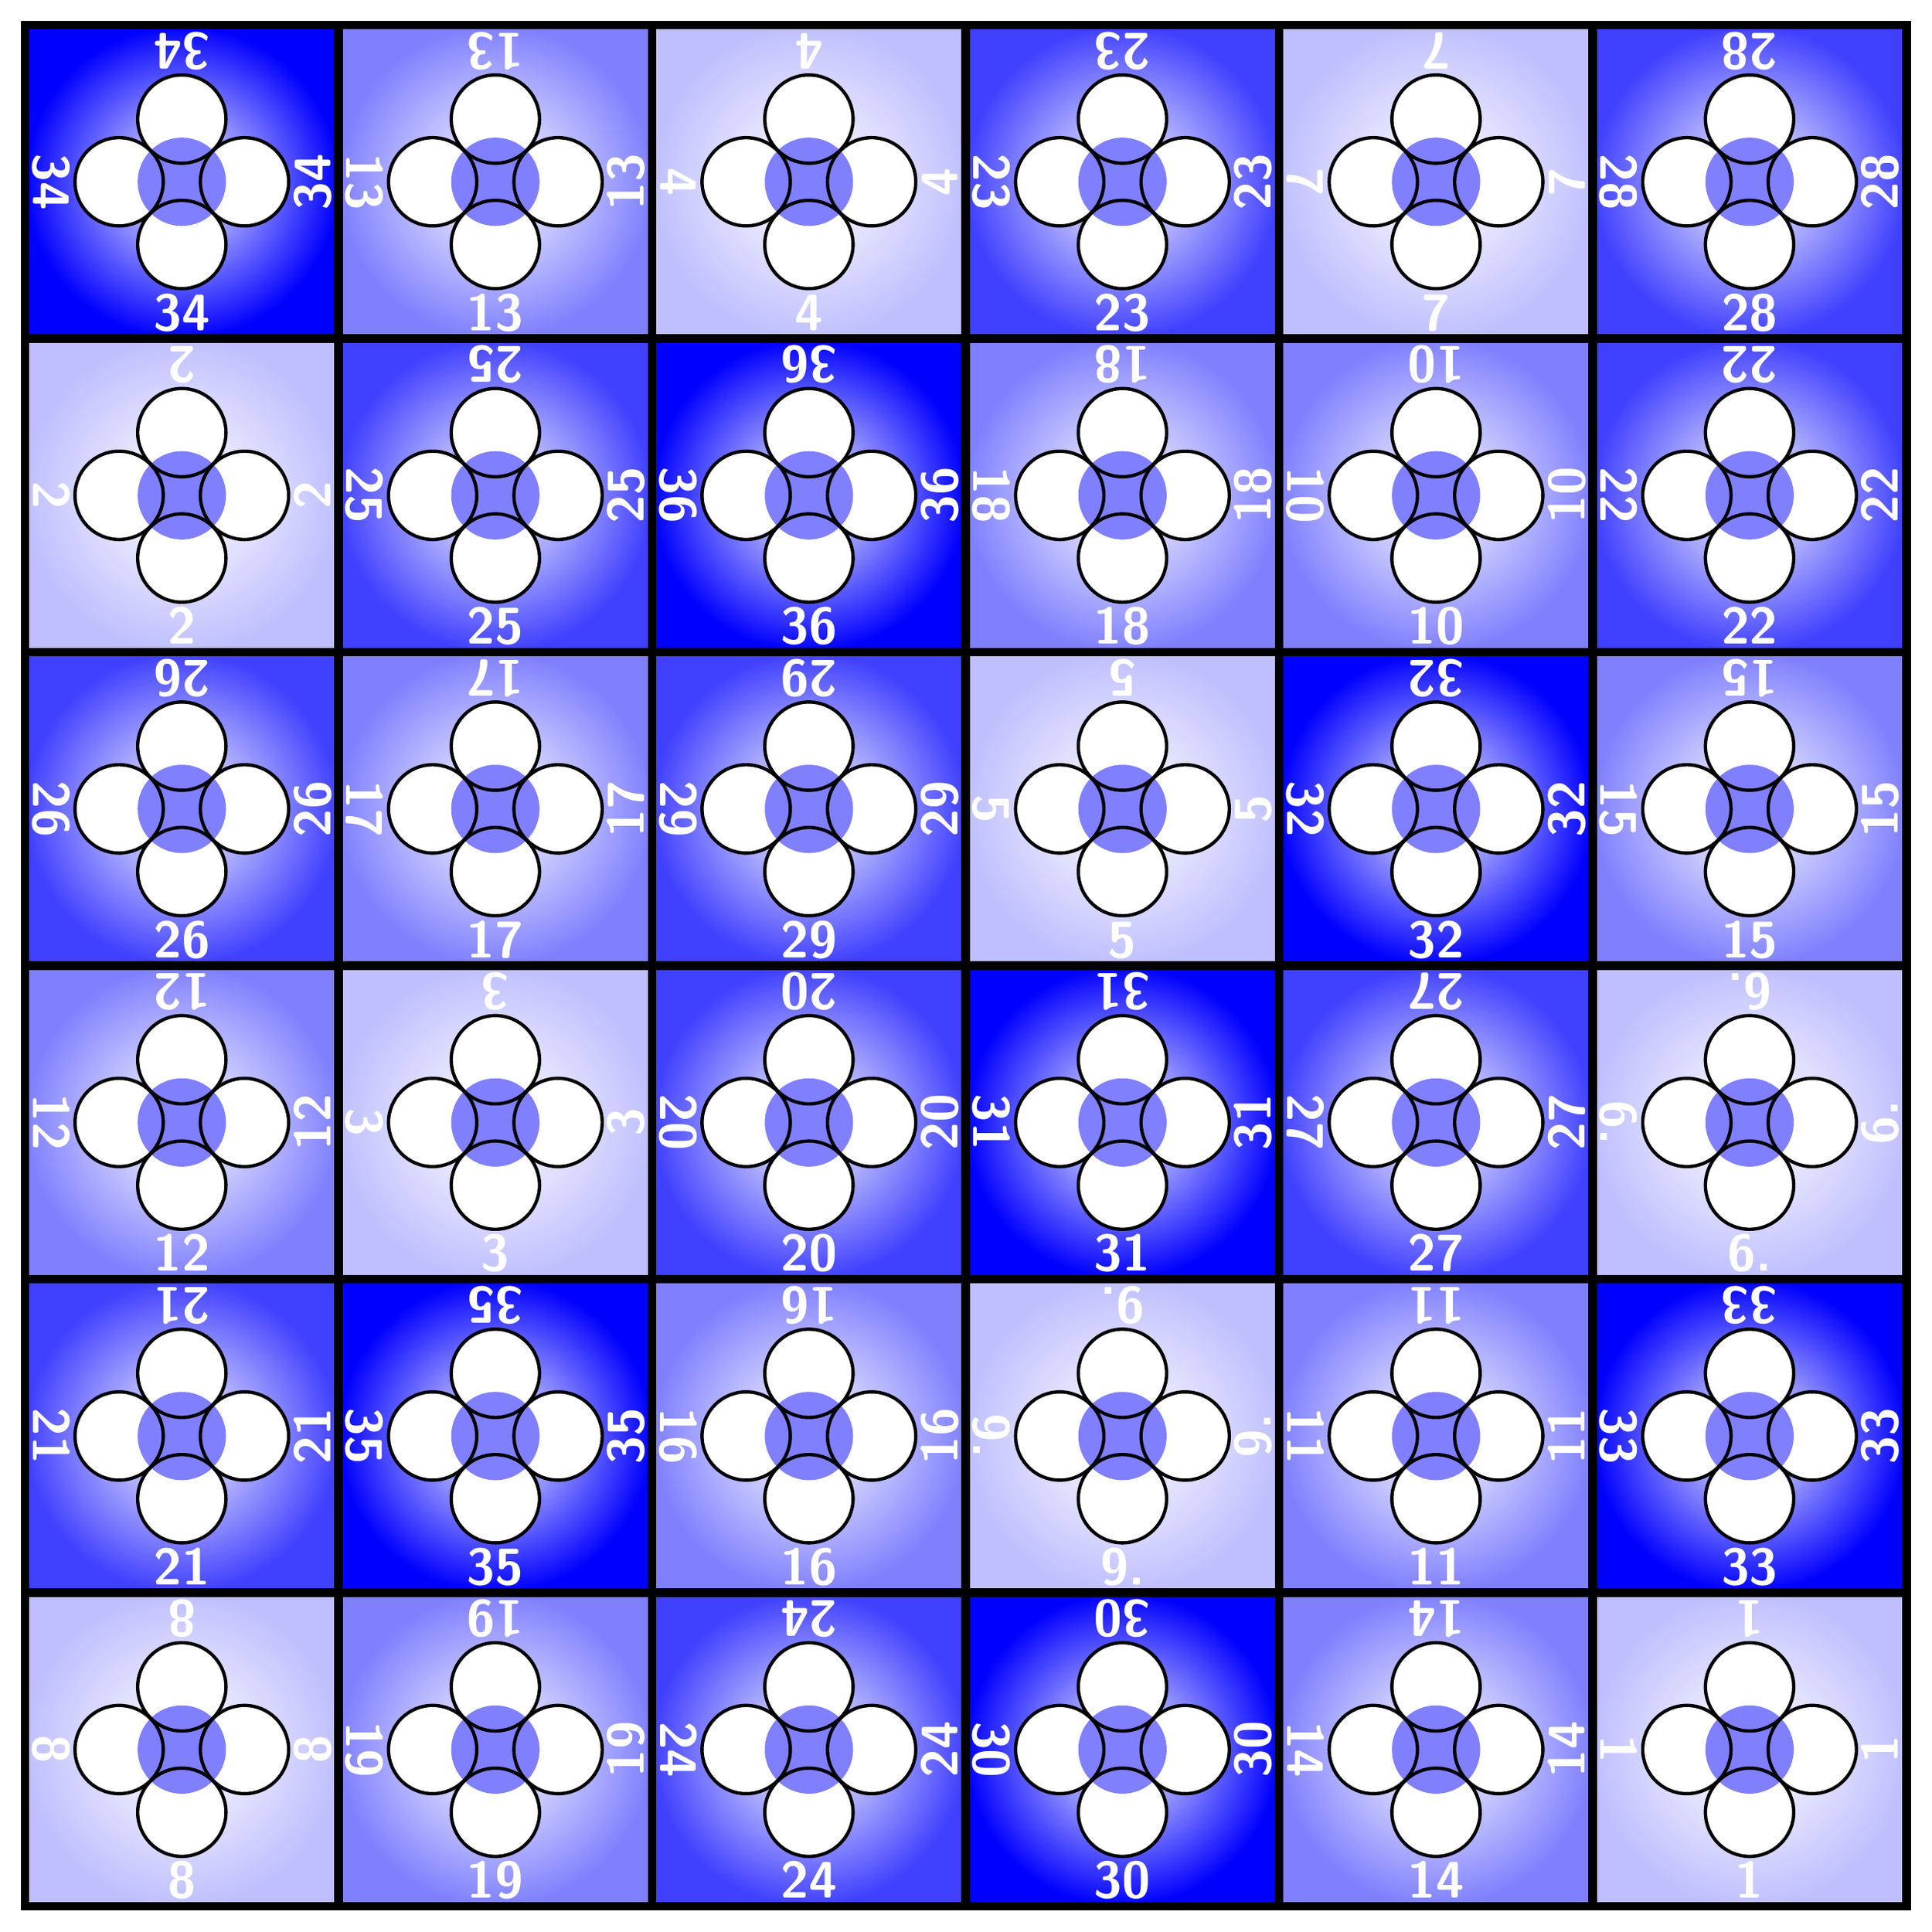
\begin{tikzpicture}[font=\sffamily]
    	\def\nums{%
    	    { 8,19,24,30,14, 1,%
			 21,35,16,9.,11,33,%
			 12, 3,20,31,27,6.,%
			 26,17,29, 5,32,15,%
			  2,25,36,18,10,22,%
			 34,13, 4,23, 7,28 %
			}};
    	\foreach \x in {0,...,5} {
    		\foreach \y in {0,...,5} {
    			{\pgfmathparse{(floor((\nums[\x+6*\y]/10))+1)*25};
    			\shade [ inner color = white, outer color = blue!\pgfmathresult!white, shading=radial] (\x*\bs-\bs/2,\y*\bs-\bs/2) -- ++(0,\bs) -- ++(\bs,0) -- ++(0,-\bs) -- cycle;
    			\draw [black, line width=\base/6] (\x*\bs-\bs/2,\y*\bs-\bs/2) -- ++(0,\bs) -- ++(\bs,0) -- ++(0,-\bs) -- cycle;
        		}
        		\node (ce\x\y) [place={white}{none}] at (\x*\bs+\base+\dx,\y*\bs          ) {};
        		\node (cn\x\y) [place={white}{none}] at (\x*\bs,          \y*\bs+\base+\dx) {};
        		\node (cw\x\y) [place={white}{none}] at (\x*\bs-\base-\dx,\y*\bs          ) {};
        		\node (cs\x\y) [place={white}{none}] at (\x*\bs,          \y*\bs-\base-\dx) {};
        		\node [place={blue!50!}{none}] at (\x*\bs,\y*\bs) {};
        		\node [place={none}{black}] at (ce\x\y) {};
        		\node [place={none}{black}] at (cn\x\y) {};
        		\node [place={none}{black}] at (cw\x\y) {};
        		\node [place={none}{black}] at (cs\x\y) {};
        		{\pgfmathparse{\nums[\x+6*\y]};
        		\node [rotate= 90, text=white, yshift=1pt] at (ce\x\y.east)  {\textbf{\Huge\pgfmathresult}};
        		\node [rotate=180, text=white, yshift=1pt] at (cn\x\y.north) {\textbf{\Huge \pgfmathresult}};
        		\node [rotate=-90, text=white, yshift=1pt] at (cw\x\y.west)  {\textbf{\Huge\pgfmathresult}};
        		\node [rotate= 00, text=white, yshift=1pt] at (cs\x\y.south) {\textbf{\Huge\pgfmathresult}};
        		}
        	};
        };
    \end{tikzpicture}
\end{document}